\documentclass[tikz,border=2pt]{standalone}
\usetikzlibrary{arrows.meta}
\tikzset{sym/.style={line width=2pt, draw=black, line cap=round, line join=round}}
\begin{document}
% Lesson 1 The water cycle: cloud, rain, sea and a rising arrow
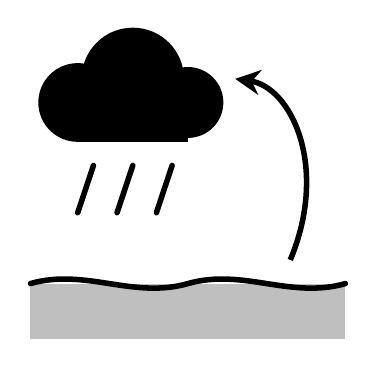
\begin{tikzpicture}
  \fill[black] (0.6,3.0) circle (0.5); \fill[black] (1.3,3.3) circle (0.65); \fill[black] (2.0,3.0) circle (0.45); \fill[black] (0.6,2.5) rectangle (2.0,3.0);
  \foreach \x in {0.8,1.3,1.8}{\draw[sym] (\x,2.2) -- (\x-0.2,1.6);}
  \fill[black!25] (0,0) rectangle (4,0.7);
  \draw[sym] (0,0.7) .. controls (0.7,0.9) and (1.3,0.5) .. (2,0.7) .. controls (2.7,0.9) and (3.3,0.5) .. (4,0.7);
  \draw[black, line width=2pt, -{Stealth[length=9pt,width=9pt]}] (3.3,1.0) .. controls (3.8,2.2) and (3.3,3.2) .. (2.6,3.3);
\end{tikzpicture}
% Lesson 3 Resources: a hill with a mine shaft, and a tree
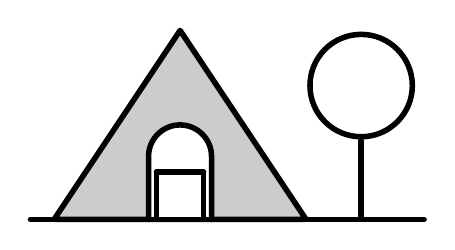
\begin{tikzpicture}
  \draw[sym, fill=black!20] (0,0) -- (1.6,2.4) -- (3.2,0) -- cycle;
  \draw[sym, fill=white] (1.2,0) -- (1.2,0.8) arc[start angle=180,end angle=0,radius=0.4] -- (2.0,0);
  \draw[sym] (1.3,0.0) -- (1.3,0.6) (1.9,0.0) -- (1.9,0.6) (1.3,0.6) -- (1.9,0.6);
  \draw[sym] (3.9,0) -- (3.9,1.0);
  \draw[sym, fill=white] (3.9,1.7) circle (0.65);
  \draw[sym] (-0.3,0) -- (4.7,0);
\end{tikzpicture}
% Lesson 4 Sustainability: three chasing arrows
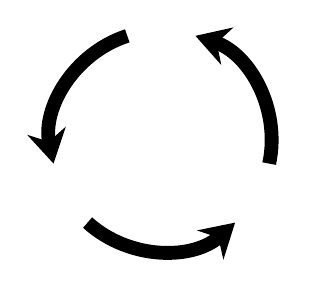
\begin{tikzpicture}
  \foreach \a in {90,210,330}{
    \draw[black, line width=5pt, -{Stealth[length=12pt,width=14pt]}] (\a+18:1.4) arc[start angle=\a+18, end angle=\a+102, radius=1.4];}
\end{tikzpicture}
% Lesson 5 Energy: a wind turbine and the sun
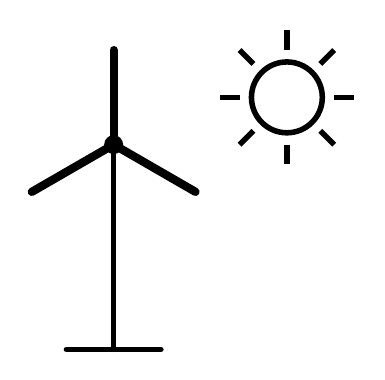
\begin{tikzpicture}
  \draw[sym] (1.4,0) -- (1.4,2.6);
  \fill (1.4,2.6) circle (0.12);
  \foreach \a in {90,210,330}{\draw[black, line width=3pt, line cap=round] (1.4,2.6) -- ++(\a:1.2);}
  \draw[sym] (0.8,0) -- (2.0,0);
  \draw[sym, fill=white] (3.6,3.2) circle (0.45);
  \foreach \a in {0,45,...,315}{\draw[black, line width=2pt] (3.6,3.2) ++(\a:0.6) -- ++(\a:0.25);}
\end{tikzpicture}
\end{document}
